%========================================================================================
% Compilation should work with PDFLaTeX
%========================================================================================
% Type of document and general formatting
\documentclass[a4paper,11pt]{article}

\usepackage[left=2.5cm,right=2.5cm,top=2.5cm,bottom=2.5cm]{geometry}
\linespread{1.25}

%========================================================================================
% These packages are for language and font settings
\usepackage[english,activeacute]{babel} % Language
\usepackage{tgpagella}					% Text font
\usepackage[T1]{fontenc}				% T1 Encoding of font
\usepackage[utf8]{inputenc}				% Special symbols
\usepackage{lmodern}


%========================================================================================
\usepackage[sc]{mathpazo}				% Math font
\usepackage{amsmath,amsfonts,amssymb}	% Math symbols
\usepackage{dsfont}						% Math symbols like R for reals...
\usepackage{amsthm}						% For theorem styles
\usepackage{siunitx}

%========================================================================================
% Other packages
\usepackage{graphicx}
\usepackage{longtable}
\usepackage[svgnames]{xcolor}

%========================================================================================
\usepackage{accents}
\newcommand*{\dt}[1]{%
	\accentset{\mbox{\large\bfseries .}}{#1}} % Larger dot for time derivative


\usepackage{hyperref}
\hypersetup
{
    pdfauthor={Rafael Serrano-Quintero},
    pdfsubject={Structural Transformation in Indian Services},
    colorlinks = {true},
    linkcolor = {FireBrick},
    citecolor = {FireBrick},
    urlcolor = {RoyalBlue},
}

\usepackage{appendix}
\usepackage{marvosym}
\usepackage{enumerate} %For enumerating with letters with option [a)]
\usepackage{enumitem}
\usepackage{fancyvrb}  %To reduce font size in verbatim environment
\usepackage{epstopdf}
\usepackage[flushleft]{threeparttable}
\usepackage{pdflscape}
\usepackage{natbib}
\usepackage{subcaption}
\usepackage{booktabs}
\usepackage[super]{nth}
\usepackage{float}

\newcommand{\source}[1]{\caption*{\tiny Source: {#1}} }

%========================================================================================
% Stata Preamble for Tables
%========================================================================================

\newcommand{\sym}[1]{\rlap{#1}}% Thanks to David Carlisle

\let\estinput=\input% define a new input command so that we can still flatten the document

\newcommand{\estwide}[3]{
		\vspace{.75ex}{
			\begin{tabular*}
			{\textwidth}{@{\hskip\tabcolsep\extracolsep\fill}l*{#2}{#3}}
			\toprule
			\estinput{#1}
			\bottomrule
			\addlinespace[.75ex]
			\end{tabular*}
			}
		}	

\newcommand{\estauto}[3]{
		\vspace{.75ex}{
			\begin{tabular}{l*{#2}{#3}}
			\toprule
			\estinput{#1}
			\bottomrule
			\addlinespace[.75ex]
			\end{tabular}
			}
		}

% Allow line breaks with \\ in specialcells
	\newcommand{\specialcell}[2][c]{%
	\begin{tabular}[#1]{@{}c@{}}#2\end{tabular}}

% *****************************************************************
% Custom subcaptions
% *****************************************************************
% Note/Source/Text after Tables
\newcommand{\figtext}[1]{
	\vspace{-1.9ex}
	\captionsetup{justification=justified,font=footnotesize}
	\caption*{\hspace{6pt}\hangindent=1.5em #1}
	}
\newcommand{\fignote}[1]{\figtext{\emph{Note:~}~#1}}

\newcommand{\figsource}[1]{\figtext{\emph{Source:~}~#1}}

% Add significance note with \starnote
\newcommand{\starnote}{\figtext{* p < 0.1, ** p < 0.05, *** p < 0.01. Standard errors in parentheses.}}

% *****************************************************************
% siunitx
% *****************************************************************
\usepackage{siunitx} % centering in tables
	\sisetup{
		detect-mode,
		tight-spacing           = true,
		group-digits            = false ,
		input-signs             = ,
		input-symbols           = ( ) [ ] - + *,
		input-open-uncertainty  = ,
		input-close-uncertainty = ,
		table-align-text-post   = false
        }

% Document parameters
\title{Chapter 2: Derivatives}
\author{Rafael Serrano Quintero \\
Dpt. Fundamentos del An\'alisis Econ\'omico \\
University of Alicante}
\date{}     

\theoremstyle{definition}
\newtheorem{definition}{Definition}
\newtheorem{example}{Example}
\theoremstyle{plain}
\newtheorem{theorem}{Theorem}
\newtheorem{lemma}{Lemma}
%========================================================================================
					% === Title, thanks, and author data === %
%========================================================================================

\begin{document}      

\maketitle

\section{Derivatives}\label{derivatives}

\subsection{Definition of Derivative}\label{definition-of-derivative}

\subsubsection{Definition and Intuition}\label{definition-and-intuition}

Let us recap from previous chapter. We have seen that the slope of a
linear function \(f(x)\) tells us the amount by which \(f(x)\) increases
given an increase in \(x\) of \(1\) unit. We also saw some economic
examples of this concept, however, it would be useful to define it for
\textbf{non-linear} functions as well.

Take the Cobb-Douglas production function defined in intensive units,
\(F(k) = k^{\alpha}\), where \(k\) is the capital-labor ratio. How could
we know how much production increases given an increase of one unit in
the capital to labor ratio? That question can be addressed by using
derivatives. The basic intuition of a derivative is the \emph{rate of
change} of a function with respect to a variable.

Suppose now we are studying a \textbf{non-linear} function \(y = f(x)\)
and that currently we are at the point \(\left(x_0, f(x_0)\right)\) on
the graph of \(f\). If we want to measure the rate of change of \(f\) or
the steepness of the graph of \(f\) when \(x = x_0\) we could simply
draw the tangent line to the graph of \(f\) at \(x_0\), since the
tangent line approximates very closely the graph of \(f\)
\textbf{around} the point \(\left(x_0, f(x_0)\right)\). Thus, the slope
of the tangent line would be a good approximation for the rate of change
of \(f\) at that point.

    \begin{figure}[htbp]
    	\centering 
    		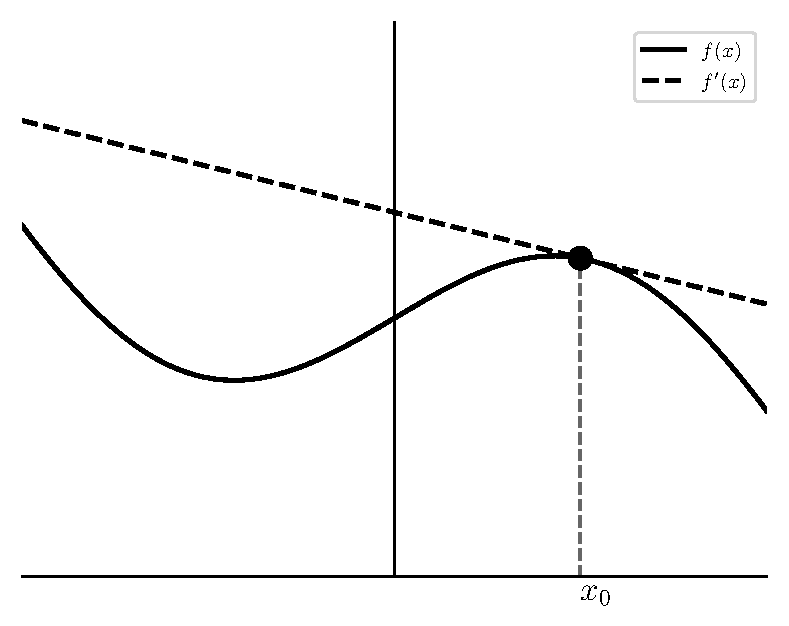
\includegraphics[width = 0.65\textwidth]{Ch2_files/Ch2_1_0.pdf}
    \end{figure}
    
    So, the slope of a non-linear function \(f\) at a point
\(\left(x_0,f(x_0)\right)\) on its graph is the slope of the tangent
line to the graph of \(f\) at that point. The \textbf{slope} of the
tangent line to the graph of \(f\) at \(\left(x_0,f(x_0)\right)\) is
called the \textbf{derivative} of \(f\) at \(x_0\).

However, we still lack a precise definition of \emph{tangent line}. Let
us start by defining a \emph{secant line}.

Consider a function \(f : \mathcal{D}\rightarrow\mathbb{R}\) and two
points in its graph,
\(\left(x_0, f(x_0)\right),\left(x_1, f(x_1)\right)\). The line segment
that joins these two points is called a \emph{secant line}. From
previous chapter, we can then define:

\[
y_1 - y_0 = m(x_1 - x_0) \ ; \  m = \frac{y_1 - y_0}{x_1 - x_0}
\]

Let us now back off a bit from \(\left(x_0, f(x_0)\right)\) to
\(\left(x_0+h_1, f(x_0+h_1)\right)\) where \(h_1\) is some small number.
And let us draw a line \(\ell_1\) joining these two points as in the
following figure. Then, \(\ell_1\) is an approximation to the tangent.
Choose a smaller \(h_2\) and draw the secant line (\(\ell_2\)) and
repeat this procedure by choosing a sequence \(\{h_n\}\) of small
numbers converging monotonically to \(0\). For each \(n\), draw a secant
line \(\ell_n\) through the distinct points on the graph
\(\left(x_0, f(x_0)\right)\) and \(\left(x_0+h_n, f(x_0+h_n)\right)\).
The secant lines \(\{\ell_n\}\) geometrically approach the tangent line
to the graph of \(f\) at \(\left(x_0, f(x_0)\right)\) and their slopes
approach the slope of the tangent line.

Since \(\ell_n\) passes through the two points
\(\left(x_0, f(x_0)\right)\) and \(\left(x_0+h_n, f(x_0+h_n)\right)\)
its slope is:

\[
\frac{f(x_0 + h_n) - f(x_0)}{(x_0+h_n)-x_0} = \frac{f(x_0 + h_n) - f(x_0)}{h_n}
\]

Thus, the slope of the tangent line is the limit of this process as
\(h_n\) converges to \(0\). Note that this is a process occurring in the
\emph{limit}, it is an infinite sequence of lines \(\ell_n\) that appear
as \(h_n\) is becoming each time smaller and smaller.

    \begin{figure}[htbp]
    	\centering 
    		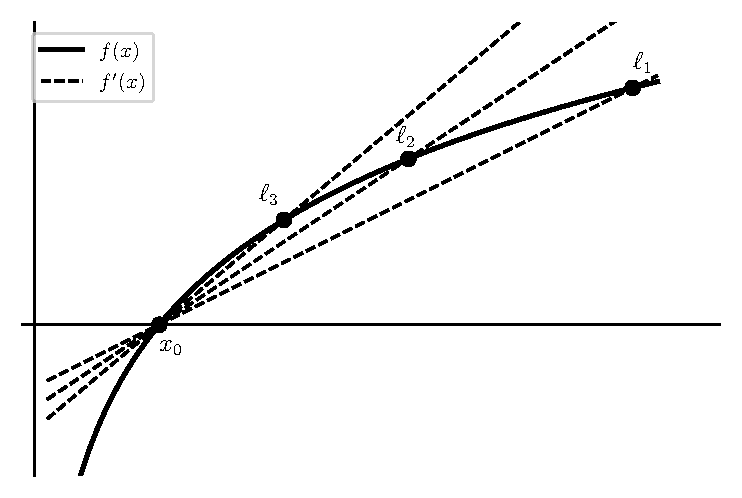
\includegraphics[width = 0.65\textwidth]{Ch2_files/Ch2_3_0.pdf}
    \end{figure}

\begin{definition}
Let \(\left(x_0, f(x_0)\right)\) be a point on the
graph of \(y = f(x)\). The \textbf{derivative} of \(f\) at \(x_0\)
denoted by

\[
f'(x_0) \ \text{or } \frac{df}{dx}(x_0) \ \text{or } \frac{dy}{dx}(x_0)
\]

is the slope of the tangent line to the graph of \(f\) at
\(\left(x_0, f(x_0)\right)\). Analytically,

\[
f'(x_0) = \lim_{h\rightarrow 0} \frac{f(x_0 + h) - f(x_0)}{h}
\]

If the limit exists. When the limit \textbf{does exist}, we say that the
function \(f\) is \textbf{differentiable} at \(x_0\) with derivative
\(f'(x_0)\).
\end{definition}

\subsubsection{Computing a derivative using the
definition}\label{computing-a-derivative-using-the-definition}

\begin{enumerate}
\def\labelenumi{\arabic{enumi}.}
\item
  Compute the increment of the function \(f(x_0 + h) - f(x_0)\).
\item
  Compute the slope as \(\dfrac{f(x_0+h)-f(x_0)}{h}\)
\item
  Compute the limit of the slope
  \(\lim_{h\rightarrow 0}{\dfrac{f(x_0+h)-f(x_0}{h}}\)
\end{enumerate}

\textbf{Example:} Let's compute the derivative of \(f(x) = x^2\) at
\(x_0 = 3\). To choose a sequence of \(\{h_n\}\) converging to zero,
let's use

\[
\{h_n\} = 0.1, 0.01, 0.001,\ldots,(0.1)^n,\ldots
\]

\begin{table}[htbp]
\centering
\begin{tabular}{cccc}
\toprule
   $h_n$ &   $x_0+h_n$ &   $f(x_0 + h_n)$ &   $\dfrac{f(x_0 + h_n)}{h_n}$ \\ \midrule
  $0.1$    &     $3.1$     &          $9.61$    &                      $6.1$     \\
  $0.01$   &     $3.01$    &          $9.0601$  &                      $6.01$    \\
  $0.001$  &     $3.001$   &          $9.006$   &                      $6.001$   \\
  $0.0001$ &     $3.0001$  &          $9.0006$  &                      $6.0001$  \\
  $0.00001$  &     $3.00001$ &          $9.00006$ &                      $6.00001$ \\
\bottomrule
\end{tabular}
\end{table}

It is easy to show, using the steps above, that \(f'(x) = 2x\) whatever
\(x\) is. Let us show that:

\begin{enumerate}
\def\labelenumi{\arabic{enumi}.}
\item
  Increment: \[
  f(x_0 + h)-f(x_0) = (x_0+h)^2-x_0^2 = x_0^2+h^2+2x_0h-x_0^2 = 2x_0 h +h^2
  \]
\item
  Slope: \[
  \frac{f(x_0+h)-f(x_0)}{h} = \frac{2x_0 h +h^2}{h} = 2x + h
  \]
\item
  Limit: \[
  \lim_{h\rightarrow 0}{\frac{f(x_0+h)-f(x_0)}{h}} = \lim_{h\rightarrow 0}{2x+h} = 2x
  \]
\end{enumerate}

In a more general setting, let us show the following two results.

\begin{theorem}
For any positive integer \(k\), the derivative of
\(f(x) = x^k\) at \(x_0\) is \(f'(x_0) = k x_0^{k-1}\)
\end{theorem}

\begin{proof}
\begin{align*}
\frac{(x_0+h)^k-x_0^k}{h} &= \frac{x_0^k+kx_0^{k-1}h + \frac{1}{2}k(k-1)x_0^{k-2}h^2+\ldots+a_kh^k-x_0^k}{h} \\
&= \frac{h(kx_0^{k-1} + \frac{1}{2}k(k-1)x_0^{k-2}h + \ldots + a_k h^{k-1})}{h} \\
&= kx_0^{k-1}  + \frac{1}{2}k(k-1)x_0^{k-2}h + \ldots + a_k h^{k-1}
\end{align*}

Note that \[
\lim_{h\rightarrow 0}{kx_0^{k-1}  + \frac{1}{2}k(k-1)x_0^{k-2}h + \ldots + a_k h^{k-1}} = kx_0^{k-1}
\]
\end{proof}

Previous Theorem uses the \emph{binomial expansion} which we define
next.

\begin{lemma}
For any positive integer \(k\), \[
(x + h)^k = x^k + a_1 x^{k-1}h^1+\ldots+a_{k-1}x^1 h^{k-1} + a_k h^k
\]

Where

\[
a_j = \frac{k!\,}{j!\,(k-j)!\,} \ \text{for } j = 1, \ldots, k
\]

In particular, \(a_1 = k, a_2 = k(k-1) / 2\), and \(a_k = 1\).
\end{lemma}

\subsubsection{Tangent line of a graph in a
point}\label{tangent-line-of-a-graph-in-a-point}

Given a differentiable function \(f : \mathcal{D}\rightarrow\mathbb{R}\)
in a point \(x_0\in\mathcal{D}\), the tangent line to the graph in the
point \(\left(x_0, f(x_0)\right)\) can be obtained from its slope
\((m = f'(x_0))\) and the point it goes through. Thus, its equation will
be given by

\[
y - f(x_0) = f'(x_0)(x - x_0)
\]

\begin{example}
Given the function \(f(x) = x^2\) in \(x_0 = -1\):

\begin{enumerate}
\def\labelenumi{\arabic{enumi}.}
\item
  \(f'(x) = 2x\) (from before), thus \(m = f'(-1) = -2\)
\item
  To get the point, \(\left(x_0, f(x_0)\right)\), \(f(-1) = 1\).
\item
  Line that goes through \((-1,1)\) with slope \(m = -2\) is given by \[
  y-1 = (-2)(x-(-1)) \Rightarrow y = -2x -1
  \]
\end{enumerate}
\end{example}

\subsection{Interpretation of the
Derivative}\label{interpretation-of-the-derivative}

We have said before that the derivative is a \emph{rate of change}, more
precisely, an \emph{instantaneous rate of change} or growth of a
function. As you will see, this concept is of crucial importance in
economics.

\subsubsection{Macroeconomics}\label{macroeconomics}

A production function of central importance in macroeconomics is the
Cobb-Douglas production function. This function relates production (GDP)
to some inputs. Suppose that the production per capita in a country is
given by the per capita machines used. That is:

\[
y = f(k) = k^{\alpha}
\]

Where \(y\) is output per capita, \(k\) is capital (machines) per
capita, and \(\alpha\in(0,1)\) is a parameter denoting the share of
income devoted to capital or capital intensity in production.

Suppose we would like to know by how much production changes if we add
\emph{an additional unit of capital per person}. That is given precisely
by the concept of derivative. As we have proved before, the derivative
of this production function is given by:

\[
f'(k) = \alpha k^{\alpha-1}
\]

Let's represent the production function and its derivative to draw some
conclusions.

    \begin{figure}[htbp]
    	\centering 
    		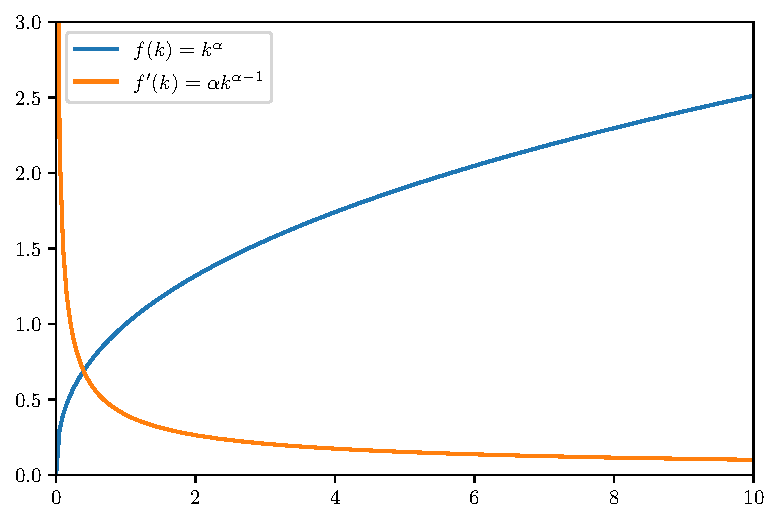
\includegraphics[width = 0.65\textwidth]{Ch2_files/Ch2_7_0.pdf}
    \end{figure}
    
    The graphs tell us that production increases with each unit of capital,
but its derivative is downward sloped, which indicates that the
\emph{rate of growth} of production with each additional unit of capital
is smaller.

This is the concept of diminishing returns to capital. When an economy
does not have many machines per person, each additional one increases
production per capita by a bigger fraction than when the economy has
lots of machines per person. This is indicated by the derivative.

In the limit, when \(k\rightarrow\infty\) production will not rise.

\subsubsection{Microeconomics}\label{microeconomics}

In theory of the firm in microeconomics, we typically deal with average
and marginal costs. A cost function \(c(q)\) indicates how much is the
cost of producing \(q\) units of a certain good. The \emph{marginal
cost} is the cost of producing an additional unit of the good. Average
cost, instead, is defined as the total cost of producing \(q\) units
divided by the \(q\) units so, it would give the cost per unit produced
of the good.

Suppose the cost function is given by

\[
c(q) = bq^2 + cq + d
\]

Where \(b, c,\) and \(d\) are constant parameters. The marginal cost can
be computed as:

\begin{enumerate}
\def\labelenumi{\arabic{enumi}.}
\item
  Compute the increment: \[
  c(q+h)-c(q) = bh^2 + b2qh + ch
  \]
\item
  Compute the slope: \[
  \frac{c(q+h)-c(q)}{h} = \frac{bh^2 + b2qh + ch}{h} = bh + 2bq + c
  \]
\item
  Compute the limit: \[
  \lim_{h\rightarrow 0}{\frac{c(q+h)-c(q)}{h}} = \lim_{h\rightarrow 0}{bh + 2bq + c} = 2q + c
  \]
\end{enumerate}

Thus, the cost of an additional unit produced is \(2q + c\) regardless
of the amount produced \(q\). However, the average cost is given by

\[
\frac{c(q)}{q} = bq + c + \frac{d}{q}
\]

Coefficient \(d\) can be interpreted as a \emph{sunk cost} which is a
cost that you need to pay regardless of the amount you produce. Notice
that coefficient \(d\) does \textbf{not} affect the marginal cost, but
it does affect the \emph{average} cost. Can you rationalize that?

\section{Rules for Computing
Derivatives}\label{rules-for-computing-derivatives}

Recall the notation. If we assume \(f(x) = x^3\) and \(g(x) = 6x^2\)

\begin{enumerate}
\def\labelenumi{\arabic{enumi}.}
\item
  \[(f + g)(x) = f(x) + g(x) = x^3 + 6x^2\]
\item
  \[(f\cdot g)(x) = f(x)\cdot g(x) = x^3 6x^2 = 6x^5\]
\item
  \[\left(\frac{f}{g}\right) = \frac{f(x)}{g(x)} = \frac{x^3}{6x^2} = \frac{1}{6}x\]
\end{enumerate}

\begin{theorem}\label{thm:deri_rules}
Suppose that \(k\) is an arbitrary constant and that
\(f\) and \(g\) are differentiable functions at \(x = x_0\). Then:

\begin{enumerate}
\def\labelenumi{\arabic{enumi}.}
\item
  \[(f\pm g)'(x_0) = f'(x_0) + g'(x_0)\]
\item
  \[(kf)'(x_0) = k\left(f'(x_0)\right)\]
\item
  \[(f\cdot g)'(x_0) = f'(x_0)g(x_0) + f(x_0)g'(x_0)\]
\item
  \[\left(\frac{f}{g}\right)'(x_0) = \frac{f'(x_0)g(x_0) - f(x_0)g'(x_0)}{g(x_0)^2}\]
\item
  \[\left(\left(f(x)\right)^n\right)' = n\left(f(x)\right)^{n-1}\cdot f'(x)\]
\item
  \[\left(x^k\right)' = kx^{k-1}\]
\end{enumerate}
\end{theorem}

\begin{proof}[\textbf{Sketch of the Proof:}]
Parts \(1\) and \(2\) are straightforward
to obtain by using the definition of derivative. Part \(3\) is obtained
by using the definition and using \(f(x_0)g(x_0+h) - f(x_0)g(x_0+h)\) in
the numerator to factor and use the properties of limits to get the
result. Part \(4\) is almost analogous to Part \(3\) just applying
properties of limits. Part \(5\) is a bit more tricky, prove it first for the case of $n = 2$, prove it then for $(n+1)$; since you proved it for any integer $n$ and any other integer $n+1$, the proof is complete. Part \(5\) is a particular case of the \textbf{Chain Rule} below.
\end{proof}

\textbf{Chain Rule:} The derivative of the composite function
\((f\circ g)(x) = f(g(x))\) is given by: \[
\left(f\circ g\right)'(x) = g'(x)f'\left(g(x)\right)
\]

\subsubsection{Derivatives of other Elemental
Functions}\label{derivatives-of-other-elemental-functions}

\begin{itemize}
\item
  Natural log: \[\left(\ln(x)\right)' = \frac{1}{x}\]
\end{itemize}

\begin{proof}
Let's start from the definition of the derivative:

\begin{align*}
f'(x_0) &= \lim_{h\rightarrow 0}{\frac{f(x_0+h)-f(x_0)}{h}} \\
&= \lim_{h\rightarrow 0}{\frac{\ln(x_0+h)-\ln(x_0)}{h}} \\
&= \lim_{h\rightarrow 0}{\frac{\ln\left(\frac{x_0 + h}{x_0}\right)}{h}} \\
&= \lim_{h\rightarrow 0}{\frac{1}{h}\ln\left(1+\frac{h}{x_0}\right)} \\
&= \lim_{h\rightarrow 0}{\left(1+\frac{h}{x_0}\right)^{\frac{1}{h}}} \\
\end{align*}

Let us define now:

\[
e = \lim_{h / x \rightarrow 0}{\left(1+h\right)^{\frac{x}{h}}} = \lim_{h / x\rightarrow 0}{\left(1+\frac{h}{x}\right)^{\frac{x}{h}}} = \lim_{h\rightarrow 0}{\left(1+\frac{h}{x}\right)^{\frac{x}{h}}}
\]

Where the last equality follows from the fact that
\(\frac{h}{x}\rightarrow 0\) as \(h\rightarrow 0\) since \(x\) is
constant with respect to \(h\).

Going back to the derivative, we can state that:

\begin{align*}
f'(x_0) = \lim_{h\rightarrow 0}{\frac{1}{h}\ln\left(e^{\frac{h}{x_0}}\right)} = \lim_{h\rightarrow 0}{\frac{1}{h}\frac{h}{x_0}\underset{=1}{\underbrace{\ln(e)}}} = \lim_{h\rightarrow 0}{\frac{1}{x_0}} = \frac{1}{x_0}
\end{align*}
\end{proof}

\begin{itemize}
\item
  Exponential: \[\left(e^x\right)' = e^x\]
\item
  Trigonometric: \[
  \left(\sin(x)\right)' = \cos(x) \ ; \ \left(\cos(x)\right)' = -\sin(x) \ ; \ \left(\tan(x)\right)' = \frac{1}{\left(\cos(x)\right)^2}
  \]
\end{itemize}

\section{Continuity and
Differentiability}\label{continuity-and-differentiability}

If a function \(f : \mathcal{D}\rightarrow\mathbb{R}\) is differentiable
in every \(x_0\in\mathcal{D}\) we say it is \textbf{differentiable}.
Only those functions whose graphs are \emph{smooth curves} have tangent
lines everywhere.

The following figure shows the graph for \(f(x) = \lvert x \rvert\).
Argue whether you believe the function is differentiable at \(x = 0\) or
not. Use the analytic definition of the derivative using the following
two sequences that converge to zero:

\[
h_n = \{+0.1, +0.01,+0.001,\ldots,+(0.1)^n,\ldots\}
\]

\[
k_n = \{-0.1, -0.01,-0.001,\ldots,-(0.1)^n,\ldots\}
\]

What is the result you get? What do you think that implies? Recall from
the previous Chapter on limits, what is the implication for a limit when
its value is different when it is computed \emph{from the left} and
\emph{from the right}?

    \begin{figure}[htbp]
    	\centering 
    		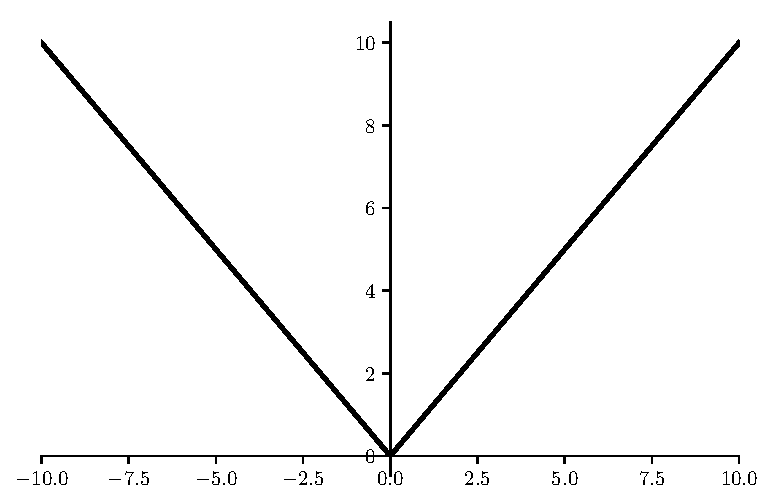
\includegraphics[width = 0.65\textwidth]{Ch2_files/Ch2_9_0.pdf}
    \end{figure}
    
    \subsection{Continuous Functions}\label{continuous-functions}

Geometrically, a function is \textbf{continuous} if it shows \emph{no
break points}. Is the previous function \(f(x) = \lvert x \rvert\)
continuous? What about \(g(x)\) defined as follows?

\[
g(x) = \begin{cases}
x\phantom{^2}+1 & x \geq 0 \\
x^2-1 & x < 0 
\end{cases}
\]

    \begin{figure}[htbp]
    	\centering 
    		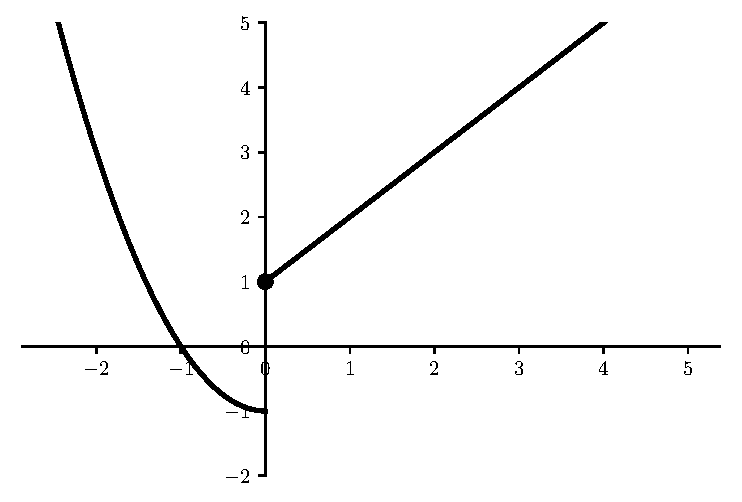
\includegraphics[width = 0.65\textwidth]{Ch2_files/Ch2_11_0.pdf}
    \end{figure}
    
    Is it possible that this function shows a tangent line at \(x = 0\)?
What is the implication of this result? How do we connect
differentiability and continuity?

What is happening under \(g(x)\) is that even if there are points in the
\(x-\)axis that are arbitrarily close to each other, the values under
\(g\) are not close to each other. Even if \((-0.1)^n\) and \((+0.1)^n\)
are arbitrarily close to each other, \(g\left((-0.1)^n\right)\) is close
to \(-1\), while \(g\left((+0.1)^n\right)\) is close to \(1\). As \(x\)
crosses \(0\) the function takes radically different values.

Do the same exercise as for \(g(x)\) above but for:

\[
f(x) = \begin{cases}
x^3 & x>0 \\
x^2 & x\leq 0
\end{cases}
\]

    \begin{figure}[htbp]
    	\centering 
    		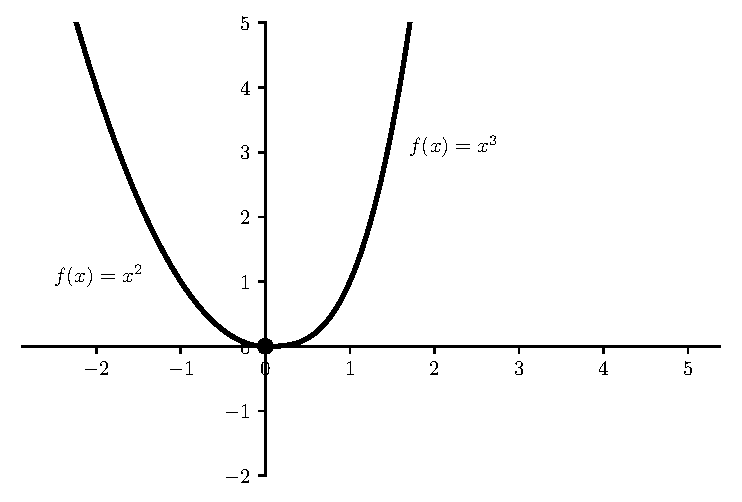
\includegraphics[width = 0.65\textwidth]{Ch2_files/Ch2_13_0.pdf}
    \end{figure}

\begin{definition}
A function \(f:\mathcal{D}\rightarrow\mathbb{R}\)
is \textbf{continuous} at \(x_0\in\mathcal{D}\) if for \emph{any}
sequence \(\{x_n\}\) that converges to \(x_0\) in \(\mathcal{D}\),
\(f(x_n)\) converges to \(f(x_0)\). A function is \textbf{continuous on
a set} \(\mathcal{U}\subset\mathcal{D}\) if it is continuous at every
\(x\in\mathcal{U}\). A function is continuous if it is continuous at
every \(x\in\mathcal{D}\).
\end{definition}

\begin{theorem}
If \(f : \mathcal{D}\rightarrow\mathbb{R}\) is
differentiable at a point \(x_0\in\mathcal{D}\), then it is also
\textbf{continuous} at that point.
\end{theorem}

\begin{proof}
For the function to be differentiable, the following
limit must exist:

\[
\lim_{h\rightarrow 0}\frac{f(x_0 + h) - f(x_0)}{h}
\]

Which implies that \(f(x_0)\) exists. To show continuity, it must be
that

\[
\lim_{x\rightarrow x_0}f(x) = \mathcal{L} = f(x_0)
\]

Therefore:

\begin{align*}
\mathcal{L} = \lim_{x\rightarrow x_0}f(x) & = \lim_{h\rightarrow 0}f(x_0 + h) \\
& = \lim_{h\rightarrow 0}f(x_0 + h)-f(x_0) + f(x_0) \\
& = \lim_{h\rightarrow 0}\left\{\frac{f(x_0+h)-f(x_0)}{h}h + f(x_0)\right\} \\
& = f'(x_0) \cdot 0 + f(x_0) = f(x_0)
\end{align*}
Thus, the function is continuous in \(x = x_0\).
\end{proof}

\begin{example}
Represent the graph of the Leontief production
function. Suppose that a firm produces using capital and labor, however,
it has a particular production structure. The firm's workers can
\emph{at most} use one machine per worker, that is, they can
\emph{share} machines or use each worker a single machine. That
production function would be given by:

\[
q = min\left\{\frac{k}{a}, \frac{1}{b}\right\}
\]

Where \(k\) is again machines per worker, \(q\) is the production per
worker of the firm, and \(a,b\) are two positive constants.

\begin{itemize}
\item
  Is it continuous?
\item
  Is it differentiable? Can we compute the \emph{marginal product} of
  capital per worker?
\item
  Can you think of an example where this production function
  \textbf{makes sense} economically?
\end{itemize}

    \begin{figure}[htbp]
    	\centering 
    		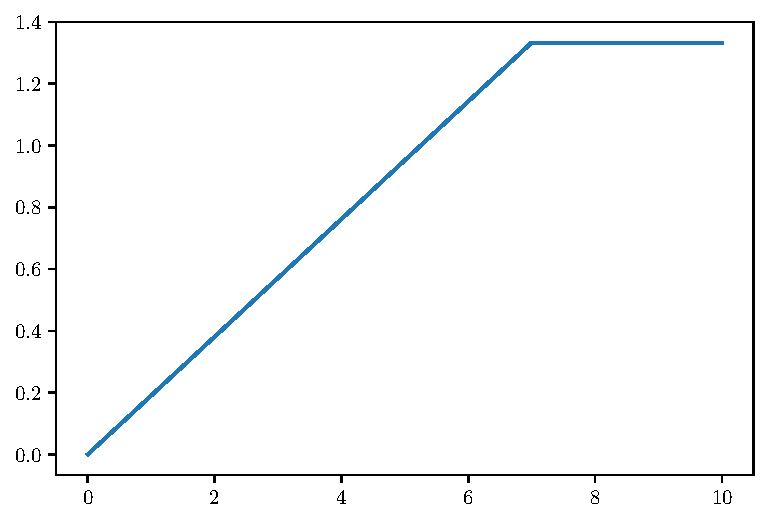
\includegraphics[width = 0.65\textwidth]{Ch2_files/Ch2_15_0.pdf}
    \end{figure}

\end{example}
    
    \section{Some Important Results}\label{some-important-results}

\begin{theorem}[\textbf{Rolle's Theorem}]
If \(f:\mathcal{D}\rightarrow\mathbb{R}\) is continuous in the closed
interval \([a,b]\subseteq\mathcal{D}\) and it is differentiable in the
open interval \((a,b)\subseteq\mathcal{D}\), and it is also fulfilled
that \(f(a) = f(b)\), then there exists \emph{at least} one point
\(c\in(a,b)\) such that \(f'(c) = 0\).
\end{theorem}

\begin{proof}
There are two possibilities, 

\begin{itemize}
    \item If \(f(x)\) is constant on \([a,b]\), then \(f'(c) = 0 \ \forall \ c\in[a,b]\). 

    \item If \(f(x)\) is \textbf{not} constant on \([a,b]\) then, by \textbf{Weierstrass' Theorem} it achieves a maximum or a minimum at some point \(c\in[a,b]\). 
\end{itemize}

Let us assume without loss of generality that \(f\) achieves a maximum. Then, for an \(h\in\mathbb{R}\) such that \((c+h)\in[a,b]\), the value \(f(c+h)\) must be smaller or equal to \(f(c)\) since \(f\) attains a maximum at \(c\). Therefore, for every \(h > 0\):

\[
\frac{f(c + h)-f(c)}{h} \leq 0
\]

Hence,

\[
f'(c+) := \lim_{h\rightarrow 0^+}{\frac{f(c+h)-f(c)}{h}} \leq 0
\]

Similarly, for every \(h < 0\):

\[
f'(c-) := \lim_{h\rightarrow 0^-}{\frac{f(c+h)-f(c)}{h}} \geq 0
\]

When these two limits agree, then the derivative of \(f\) at \(c\) must
be \(0\). Since the function is continuous in \([a,b]\) the two lateral
limtis coincide, and thus, the function is differentiable.
\end{proof}

\begin{theorem}[\textbf{L'H\^opital Theorem}]
Let \(f,g : \mathcal{D} \rightarrow \mathbb{R}\) two differentiable
functions such that \(\lim_{x\rightarrow x_0} f(x) = \lim_{x\rightarrow x_0} g(x) = 0\). If the limit \(\lim_{x\rightarrow x_0}{\frac{f'(x)}{g'(x)}}\) exists, then

\[
\lim_{x\rightarrow x_0}{\frac{f(x)}{g(x)}} = \lim_{x\rightarrow x_0}{\frac{f'(x)}{g'(x)}} = \mathcal{L}
\]
\end{theorem}

What this result shows is that, in certain limits, the functions can be
replaced by their derivatives. To grasp the idea, it is as if we would
change the functions by their slopes, in some way, it is a linear
approximation.

The importance of this theorem comes also from the fact that it allows
us to compute limits in which indeterminations appear. The following two
examples show the power of this theorem.

\begin{example}
Compute the limit of

\begin{itemize}
\item
  \[\lim_{x\rightarrow 0}{\frac{\sin(x)}{x}}\]
\end{itemize}

It is clear that by substituting \(x = 0\) in the limit we obtain an
indetermination. However, taking the derivative of the numerator and the
denominator separately:

\[
\lim_{x\rightarrow 0}{\frac{\cos(x)}{1}} = 1
\]

\begin{itemize}
\item
  \[\lim_{x\rightarrow 0}{\frac{x}{e^x}}\]
\end{itemize}

This second case is a bit more intuitive since the exponential function
grows faster than the linear function, so the denominator will go faster
to infinity than the numerator, which implies this limit is \(0\). Using
L'Hôpital's Theorem:

\[
\lim_{x\rightarrow +\infty}{\frac{1}{e^x}} = \frac{1}{+\infty} = 0
\]

\begin{itemize}
\item
  \[\lim_{x\rightarrow +\infty}{\left(1 + \frac{1}{x}\right)^x}\]
\end{itemize}

This is a more complicated limit since it would yield \(1^{\infty}\),
which is an indetermination. To deal with this type of limits, it is
possible to transform them using the log of it. Thus, let

\[
k = \lim_{x\rightarrow +\infty}{x\ln\left(1 + \frac{1}{x}\right)} = \lim_{x\rightarrow +\infty}{\frac{\ln\left(1 + \frac{1}{x}\right)}{\frac{1}{x}}} = \frac{0}{0}
\]

This yields another indetermination, but now it is possible to use
L'Hôpital's theorem.

\[
k = \lim_{x\rightarrow +\infty}{\frac{\frac{-\frac{1}{x^2}}{1 + \frac{1}{x}}}{-\frac{1}{x^2}}} = \lim_{x\rightarrow +\infty}{\frac{1}{1 + \frac{1}{x}}} = 1
\]

Note however, that \(k = 1\) is not the original limit but the
\textbf{logarithm of the original limit}, thus, the actual value of the
original limit is \(e^k = e\).
\end{example}

\section{Implicit Differentiation}\label{implicit-differentiation}

Typically, we work with \emph{explicit} functions. That is, functions
whose endogenous variables are explicit functions of the exogenous ones,
i.e.

\[
y = F(x)
\]

Sometimes, however, functions may arise as \textbf{implicit} functions.
That is, of the form:

\[
G(x, y) = 0
\]

This function \(G(\cdot)\) defines de endogenous variable \(y\) as an
\textbf{implicit function} of \(x\).

\begin{example}
When working with lines, we might have

\[
4x + 2y = 5 \ ; \ 4x + 2y - 5 = 0
\]

Which expresses \(y\) as an implicit function of \(x\). However, we can
rearrange terms so that we have an \emph{explicit} function of \(x\):

\[
y = 2.5 - 2x 
\]
\end{example}

\begin{example}
It is not always possible to transform an implicit
function into an explicit one. Consider, for example,

\[
y^5 - 2xy - 4x^2 = 0
\]

Since there is no general formula for solving an equation of \(5-\)th
degree, we cannot turn this equation into an explicit function.
Nevertheless, it does generate an implicit function of \(x\), since we
can plug any value for \(x\) and obtain a value for \(y\). Suppose
\(x = 0\), then \(y^5 = 0 \Rightarrow y = 0\).
\end{example}

Take now \(x^2 + y^2 = 1\).

\begin{itemize}
\item
  If \(x > 1\), then there is no \(y\) possible that can satisfy the
  equation.
\item
  If we start at some \((x_0, y_0)\) that is a solution to the equation,
  we can vary \(x\) a little from \(x_0\) and try to find \(y\) close to
  \(y_0\) that satisfies the equation, that would be
  \(y = \sqrt{1-x^2}\). Take \(x = 0\), thus, \(y = 1\). Then, small
  deviations from \(x = 0\) yield small deviations in \(y\) that fulfill
  the equation.
\item
  Take now, \(x = 1, y = 0\). Then, a small deviation
  \(x = 1 + \varepsilon\) there is no possible \(y\) so that
  \((1+\varepsilon,y)\) satisfies the equation.
\item
  If, instead, we deviate to \(x = 1-\varepsilon\), there are two
  possible candidates for \(y\). \[
  y = \begin{cases}
  +\sqrt{2\varepsilon-\varepsilon^2} \\
  -\sqrt{2\varepsilon-\varepsilon^2}
  \end{cases}
  \]
\end{itemize}

That is because around \((1,0)\) the curve is vertical.

    \begin{figure}[htbp]
    	\centering 
    		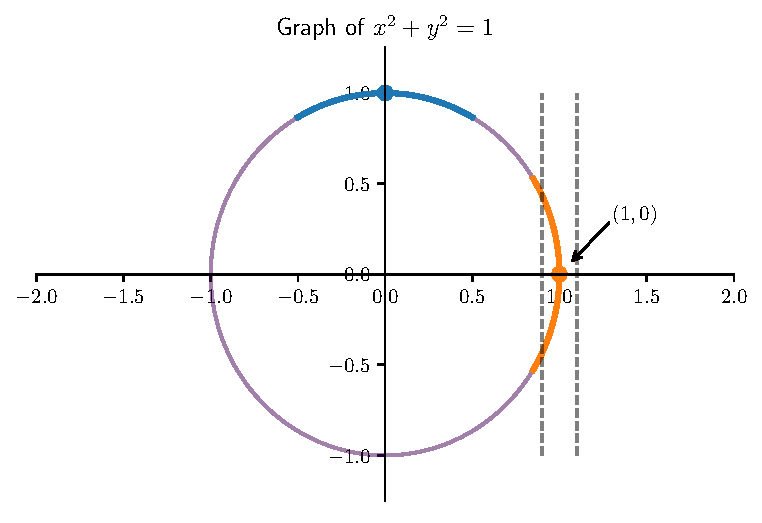
\includegraphics[width = 0.65\textwidth]{Ch2_files/Ch2_17_0.pdf}
    \end{figure}
    
    Suppose we want to know how changes in \(x\) affect the corresponding
\(y\)'s. That simply means that we want to know the change in \(y\) when
there is a given change in \(x\), which is just the derivative of \(y\)
\emph{with respect to \(x\)}.

To get the derivative of \(y\) from a given implicit function, it is
usually better to solve for \(y\) first and then take the derivative as
usual. Sometimes, as we have just seen, this is not possible but it
might be possible to find the derivative in a point where the equation
is satisfied.

Take the equation \(x-y-\ln(x)-\ln(y) = 0\). This equation is satisfied
in point \((1,1)\). So the process is about differentiating the equation
with respect to \(x\) such that we will get \(\frac{dy}{dx} = y'\) and
\(\frac{dx}{dx} = 1\). Thus, we get:

\[
1 - \frac{dy}{dx}-\frac{1}{x}-\frac{1}{y}\frac{dy}{dx} = 1 - y' - \frac{1}{x}-\frac{y'}{y} = 0
\]

Substituting now \(x = 1, y = 1\)

\[
1 - y'(1) - 1 - y'(1) = 0 \Rightarrow y'(1) = 0
\]

In the Mathematics Course you will see more on implicit differentiation.
In particular, the \textbf{Implicit Function Theorem} stated below.

\begin{theorem}[\textbf{Implicit Function Theorem}] 
Let \(G(x, y)\) be a \(\mathcal{C}^1\) (continuous and differentiable function whose first
derivatives are also continuous) function on a ball about
\((x_0, y_0)\in\mathbb{R}^2\). Suppose \(G(x_0, y_0) = c\) and consider
the expression

\[
G(x, y) = c
\]

If \(\left(\partial G / \partial y\right)(x_0, y_0) \neq 0\) then there
exists a \(\mathcal{C}^1\) function \(y = y(x)\) defined on an interval
\(\mathcal{I}\) about the point \(x_0\) such that: -
\[G\left(x,y(x)\right) = c \ \forall \ x\in\mathcal{I}\] -
\[y(x_0) = y_0\] -
\[y'(x_0) = -\frac{\frac{\partial G}{\partial x}(x_0, y_0)}{\frac{\partial G}{\partial y}(x_0, y_0)}\]
\end{theorem}

The \textbf{Implicit Function Theorem} is a central result in
mathematical analysis and of central importance for economic theory as
you will see. It gives answers to two main questions about implicit
functions:

\begin{enumerate}
\def\labelenumi{\arabic{enumi}.}
\item
  Given an implicit equation \(G(x,y) = c\) and a point \((x_0, y_0)\)
  such that the equation is satisfied, does there exist a continuous
  function \(y = y(x)\) defined on an interval \(\mathcal{I}\) about
  \(x_0\) so that
  \(G\left(x, y(x)\right) = c \ \forall \ x\in\mathcal{I}\) and for
  which \(y(x_0) = y_0\)?
\item
  If \(y(x)\) exists and is differentiable, what is \(y'(x_0)\)?
\end{enumerate}

Basically, 1 asks whether the implicit function exists and is continuous
about that point where the equation is satisfied and 2 asks for a way of
computing the derivative of this implicit function at that point where
the equation is satisfied. This theorem also exists in a multivariate
case.

\section{Maxima and Minima}\label{maxima-and-minima}

\subsection{Increasing and Decreasing
Functions}\label{increasing-and-decreasing-functions}

Recall that the definition of a derivative is the slope of the tangent
line on a point. What is the implication if the slope is positive? This
tells us that the function on that point is \emph{growing}, while if the
slope of the tangent is negative, it is telling us that the function is
\emph{decreasing} on that point. More precisely,

\begin{definition}
A function \(f(x)\) is said to be
\textbf{increasing} in an interval \([a,b]\) if: \[
\forall \ x_1,x_2\in[a,b] \ : \ x_1 < x_2 \Rightarrow f(x_1) < f(x_2)
\]

Analogously, a function is said to be \textbf{decreasing} in an interval
\([a,b]\) if:

\[
\forall \ x_1,x_2\in[a,b] \ : \ x_1 < x_2 \Rightarrow f(x_1) > f(x_2)
\]
\end{definition}

These concepts are most important in the case of non-linear functions
because straight lines are \emph{always} increasing or decreasing. Take
\(f(x) = \sin(x)\), this function will have intervals in which \(f(x)\)
increases as \(x\) increases and other intervals in which \(f(x)\)
decreases as \(x\) \emph{increases}. The following Figure helps to see
the relationship between derivatives and intervals of growth of a
function.

    \begin{figure}[htbp]
    	\centering 
    		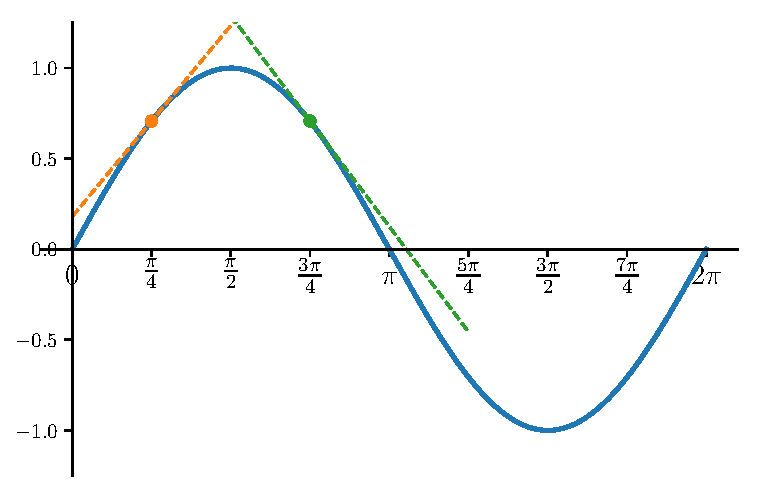
\includegraphics[width = 0.65\textwidth]{Ch2_files/Ch2_19_0.pdf}
    \end{figure}
    
    From the graph, it is easy to see the relationship between derivatives
and areas in which the function is increasing or decreasing. The
following Theorem summarizes and formalizes this idea.

\begin{theorem}
Given a function
\(f \ : \ \mathcal{D}\rightarrow\mathbb{R}\) such that
\(f\in\mathcal{C}^1\), then: 

\begin{enumerate}
    \item \(f(x)\) is \textbf{increasing} for every \(x\in\mathcal{D} \ : \ f'(x) \geq 0\) 

    \item \(f(x)\) is \textbf{decreasing} for every \(x\in\mathcal{D} \ : \ f'(x) \leq 0\)
\end{enumerate}
\end{theorem}

\subsection{Local Maxima and Minima}\label{local-maxima-and-minima}

From the discussion above, it is straightforward to see that if in a
point \(x_0\) the function achieves a \emph{local maximum}, it must be
\textbf{increasing} for those \(x < x_0\) and \textbf{decreasing} for
those \(x > x_0\). If the derivative exists and it is continuous it will
turn from being positive to being negative while in that particular
point \(x_0\) it will be \(0\). If \(x_0\) is a local minimum instead,
the reasoning is equivalent and the derivative \textbf{must also be
zero} at that point. Those points that make the first derivative \(0\)
are called \emph{critical points}.

\begin{definition}
If \(f \ : \ \mathcal{D}\rightarrow\mathbb{R}\) and
\(f\in\mathcal{C}^1\), those points for which \(f'(x) = 0\) are called
\textbf{critical or stationary points}.
\end{definition}

\begin{theorem}
If \(f \ : \ \mathcal{D}\rightarrow\mathbb{R}\) and
\(f\in\mathcal{C}^1\). Then, every point in which \(f(x)\) reaches a
local maximum or minimum are critical points. Furthermore:

\begin{itemize}
    \item If \(f'(x_0) = 0\) and the function turns from increasing to decreasing,
\(f(x)\) reaches a local maximum at \(x_0\) 

    \item If \(f'(x_0) = 0\) and the function turns from decreasing to increasing, \(f(x)\) reaches a local minimum at \(x_0\)
\end{itemize}
\end{theorem}

Note that \textbf{not every critical point must be a local maximum or
minimum}.

\begin{example}
Analyse the areas in which the function \(f(x) = x^3\)
is increasing or decreasing.

\(f'(x) = 3x^2\), so the only point for which \(f'(x) = 0\) is
\(x = 0\). However, notice that for any \(x < 0\), \(f'(x) > 0\) and so
it is for any \(x > 0\). Thus, \(x = 0\) is neither a maximum or a
minimum. This is the case of a \emph{saddle point}. Graphically:
\end{example}

    \begin{figure}[htbp]
    	\centering 
    		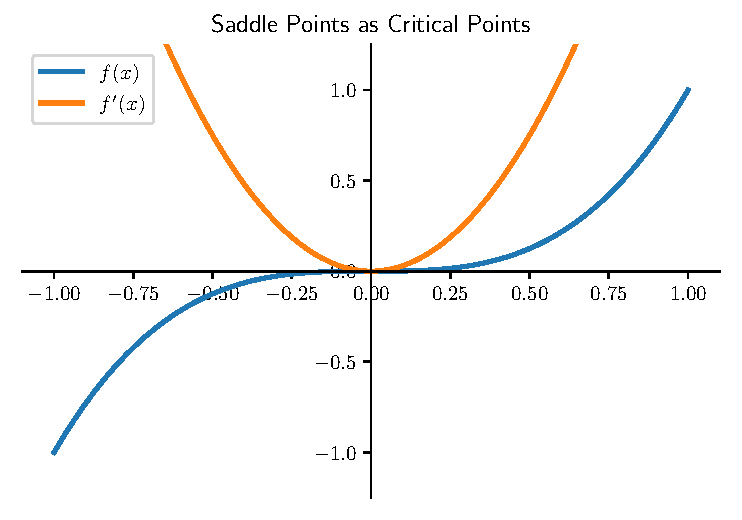
\includegraphics[width = 0.65\textwidth]{Ch2_files/Ch2_21_0.pdf}
    \end{figure}
    
    \section{Convexity and Concavity}\label{convexity-and-concavity}

Convexity and concavity refer basically to the \emph{curvature} of a
function, how the function it is shaped. Let us start with an example by
thinking about a firm's production function. Assume a firm produces with
a single input, it is reasonable to assume that the total amount of
output produced by the firm increases with this input, i.e., as we
increase the input (e.g. machines) the output of the firm will be
larger. This relates to the function being \emph{increasing} on that
input. However, as we increase the input, typically the output increases
but each time by a little less. That idea can be captured in a
production function that is both increasing in the input and also
\textbf{concave}. Suppose now that the cost of a firm is concave up to a
point in which it becomes convex. That would tell us that the cost of
producing increases each time by a smaller amount as we increase the
amount to be produced up to a point, in which the cost raises every time
faster and faster. The figure below shows both examples.

    \begin{figure}[htbp]
    	\centering 
    		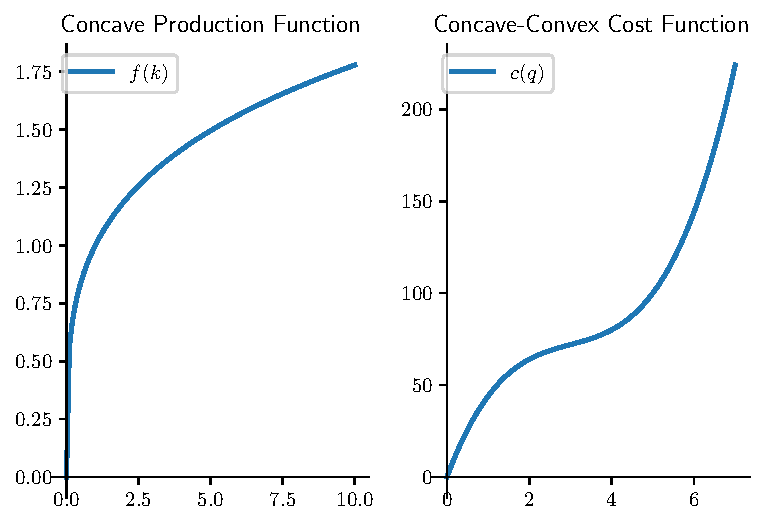
\includegraphics[width = 0.65\textwidth]{Ch2_files/Ch2_23_0.pdf}
    \end{figure}
    
    \begin{figure}[htbp]
    	\centering 
    		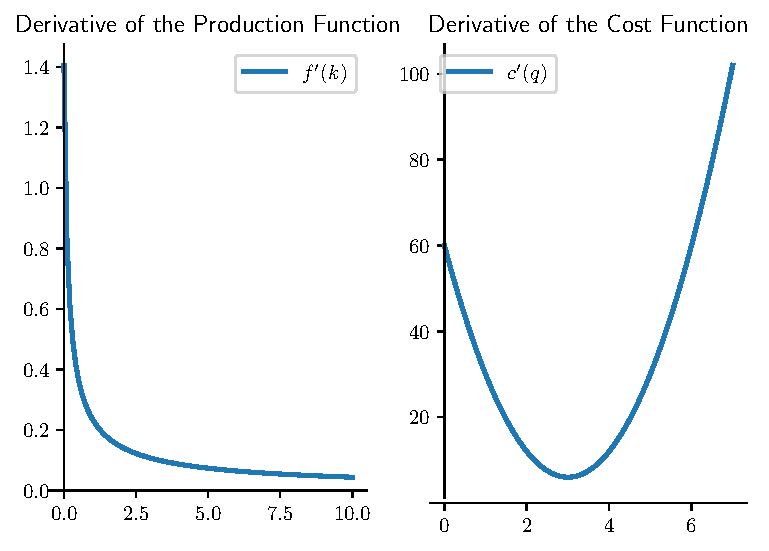
\includegraphics[width = 0.65\textwidth]{Ch2_files/Ch2_23_1.pdf}
    \end{figure}
    
    In the previous two examples, we have made reference to how much output
or cost increase given an increase in the input of the function. This is
already suggesting we should look at the derivatives of the function
since the derivative tells us precisely by how much the function
increases if the argument of the function increases (infinitesimally).

Note how the derivatives of these functions show up. For concave
functions, the derivative is decreasing, while note that for the cost
function, when it becomes convex, the derivative turns from decreasing
to increasing.

\subsection{Definition and Alternative Graph
Representation}\label{definition-and-alternative-graph-representation}

A formal definition of convexity and concavity is given below.

\begin{definition}
A function \(f \: : \: \mathcal{D} \rightarrow \mathbb{R}\) is said to be: 

\begin{itemize}
    \item \textbf{convex} in the interval \([a,b]\subseteq\mathcal{D}\) if \(\forall \: x,y\in[a,b] \: x\neq y\) and \(\forall \: \lambda\in[0, 1]\) it is fulfilled that \(f\left(\lambda x + (1-\lambda)y\right) \leq \lambda f(x) + (1-\lambda) f(y)\). It will be \emph{strictly} convex if \(f\left(\lambda x + (1-\lambda)y\right) < \lambda f(x) + (1-\lambda) f(y)\).

    \item \textbf{concave} in the interval \([a,b]\subseteq\mathcal{D}\) if \(\forall \: x,y\in[a,b] \: x\neq y\) and \(\forall \: \lambda\in[0,1]\) it is fulfilled that \(f(\lambda x + (1-\lambda) y)\geq \lambda f(x) + (1-\lambda) f(y)\). It will be \emph{strictly} concave if \(f\left(\lambda x + (1-\lambda)y\right) > \lambda f(x) + (1-\lambda) f(y)\).
\end{itemize}
\end{definition}

Note that, in general, functions do not need to be concave or convex in
all their domain (recall the example of the cost function) but they tend
to have areas of convexity and areas of concavity. These areas are
determined by the sign of the second derivative of the function.

    \begin{figure}[htbp]
    	\centering 
    		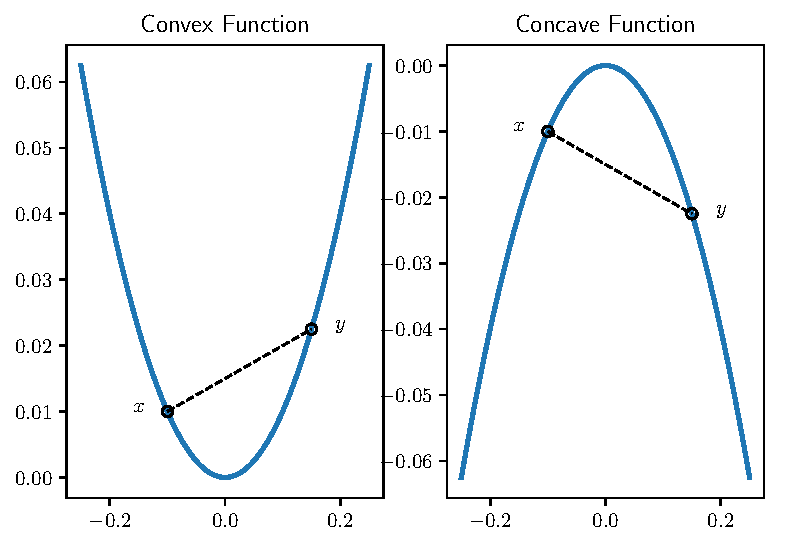
\includegraphics[width = 0.65\textwidth]{Ch2_files/Ch2_25_0.pdf}
    \end{figure}
    
    Note how the formal definition is directly related to the graphs above.
Take any \(x < z < y\), then if the point \(\left(z, f(z)\right)\) on
the graph of \(f(\cdot)\) is below (above) the segment joining
\(\left(x, f(x)\right)\) and \(\left(y, f(y)\right)\) the function is
convex (concave).

\begin{theorem}
Let \(f \: : \: \mathcal{D}\rightarrow\mathbb{R}\) be
a function with continuous first and second derivatives in all its
domain. Then: 
\begin{enumerate}
    \item \(f(x)\) is concave in \([a,b]\) if \(f''(x) \leq 0 \: \forall \: x\in[a,b]\) 
    \item \(f(x)\) is convex in \([a,b]\) if \(f''(x) \geq 0 \: \forall \: x\in[a,b]\)
\end{enumerate}
\end{theorem}

Let's build a bit of intuition on this theorem. If \(f'(x)\) measures
the \emph{rate of change} of \(f(\cdot)\), by the same token, the second
derivative measures the \emph{rate of change of the first derivative}.
Let us assume that we find a particular function whose \textbf{second}
derivative is negative. This will imply that the \emph{first} derivative
is declining, which in turn, will tell us that the function itself
increases by a lower amount with each increase in the argument. In other
words, if we have a positive \emph{first} derivative and a negative
\emph{second} derivative, that would imply that the slope of the
function is positive but \emph{decreasing} (Point \(A\) in the Figure
below). If, instead, the second derivative is \emph{positive}, the
function would have a positive and \emph{increasing} slope (Point
\(F\)).

Suppose now that the first derivative is \emph{negative}. Thus, a
\emph{positive} second derivative would tell us that the function has a
negative and \emph{increasing} slope. What does increasing mean in this
case? Precisely that the function becomes \textbf{\emph{less steep}}
since the slope would change from say, \((-5)\) to \((-2)\) (Point
\(D\)). If the second derivative is instead \emph{negative} that would
imply a function with a negative and \emph{decreasing} slope.
Analogously, in this case, \emph{decreasing} means that the function is
becoming \textbf{\emph{more steep}} (Point \(C\)).

    \begin{figure}[htbp]
    	\centering 
    		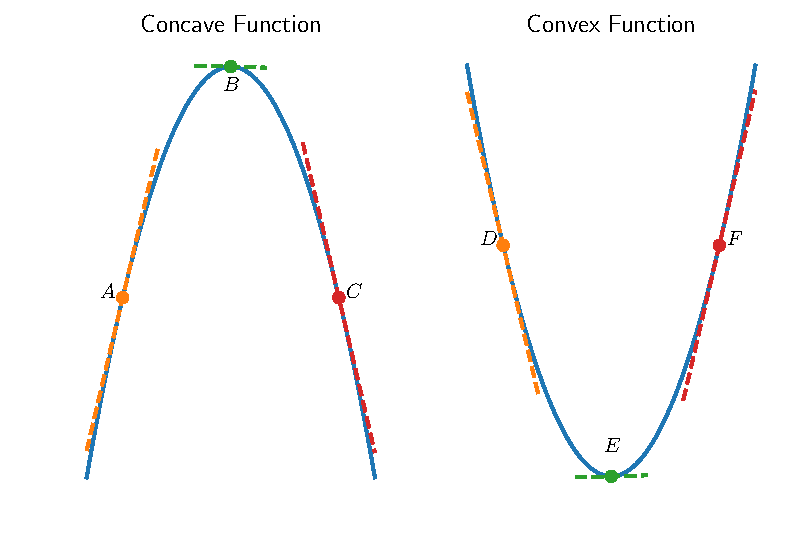
\includegraphics[width = 0.65\textwidth]{Ch2_files/Ch2_27_0.pdf}
    \end{figure}
    
    Since, in general, functions are not always concave nor convex there
must be a point in which the curvature of the function changes. That is
precisely an \textbf{\emph{inflection point}}.

\begin{definition}
it is called \textbf{inflection point} of a
function \(f \: : \: \mathcal{D}\rightarrow\mathbb{R}\) to every point
\(x\in\mathcal{D}\) in which the function changes its curvature.
\end{definition}

\subsection{Critical Points
Classification}\label{critical-points-classification}

We have seen previously how to identify whether a critical point is a
maximum or a minimum, analysing first which are the increasing and the
decreasing areas of the function. However, it is possible to check
whether a point is a maximum or a minimum through the second derivative.
It is easy to see from the graphs that, if the critical point is found
in a \emph{concave function}, then that critical point will be a
maximum. If the function is \emph{convex} instead, the critical point
will minimize the function.

\begin{theorem}
Let \(f \: : \: \mathcal{D}\rightarrow\mathbb{R}\) be
a function whose first and second derivatives are continuous in its
domain, and let \(x^*\) be a critical point of the function, i.e.
\(f'\left(x^*\right) = 0\). Then:

\begin{enumerate}
\def\labelenumi{\arabic{enumi}.}
\item
  If \(f''\left(x^*\right) > 0\) the function will reach a local minimum
  in \(x^*\).
\item
  If \(f''\left(x^*\right) < 0\) the function will reach a local maximum
  in \(x^*\).
\end{enumerate}
\end{theorem}

\section{Exercises}\label{exercises}

\begin{enumerate}
\item Compute the following limits:

    \begin{itemize}
   
    \item
    \[\displaystyle\lim_{x\rightarrow 1}{\dfrac{\log(x)}{x^2 - 1}}\]
    \item
    \[\displaystyle\lim_{x\rightarrow 0}{\dfrac{1-\cos(x)}{\sin(x)}}\]
    \item
    \[
    \lim_{x\rightarrow 0}\left(\frac{\pi}{4x} - \frac{\pi}{2x(e^{\pi x}+1)}\right)
    \]
    \end{itemize}

\item Argue whether or not the following limit is correct, which property or theorem has been used to solve it, and how has it been applied.

\[
\lim_{x\rightarrow 1}\frac{x^3+x-2}{x^2-3x+2} = \lim_{x\rightarrow 1}\frac{3x^2+1}{2x-3} = \lim_{x\rightarrow 1}\frac{6x}{2} = 3
\]

\item Prove that the derivative of a constant is zero, i.e., if $f(x) = C \: : \: C\in\mathbb{R} \Rightarrow f'(x) = 0 \: \forall \: x\in\mathbb{R}$.

\item Prove Theorem \ref{thm:deri_rules} (Parts $1$ to $4$ included) using the hints provided.


\item Prove that the derivative of the exponential function is the exponential function itself.

\item Compute the derivative of the tangent function using the quotient rule (Theorem \ref{thm:deri_rules}) and using the derivatives for the \(\sin(x)\) and \(\cos(x)\).

\item Compute the derivative of \(f(x) = \ln\left(\cos\left(x^2\right)\right)\)

\item The Constant Elasticity of Substitution production
function can be defined as:

\[
f(k) = \left(a k^{\frac{\sigma-1}{\sigma}} + (1-a)\right)^{\frac{\sigma}{\sigma-1}}
\]

Where \(k\) is the capital per person, \(a\) is a distribution
parameter, and \(\sigma\) is the elasticity of substitution between
capital and labor.

Using the rules for computing derivatives, show that
\(f'(k) = a\left(\frac{f(k)}{k}\right)^{\frac{1}{\sigma}}\).

\item Analyse the areas in which \(f(x) = 2x^2 - 1\) is
increasing and decreasing. To do so, first compute its derivative, then
compute those points for which \(f'(x) = 0\). Finally, analyse the sign
in those intervals given by the cut-points of the derivative.

\item Do the same for \(g(x) = x^3-4x^2+2\).

\item Given the function \(\displaystyle f(x) = a - \dfrac{b}{c + x} \: (a,b,c > 0; \: x \geq 0)\), determine the general shape of its graph by examining \(a)\) the domain of the function, \(b)\) cut points with the axes, \(c)\) behavior in \(x\rightarrow \pm \infty\), \(d)\) continuity, \(e)\) first and second derivatives analysis. How would you restrict the parameters of the function if this needs to be a \textbf{consumption}function?

\item Verify whether the following functions fulfill the requirements of Rolle's theorem.

    \begin{enumerate}[label = (\alph*)]
        \item \(f(x) = x^3 - 9x + 1\) for the intervals \([-3,3],[0, 3]\), and \([0, 1]\).
        \item \(f(x) = \lvert x \rvert\) for the interval \([0, 1]\).
    \end{enumerate}

\item Suppose a \textbf{profit maximizing} firm has a revenue function \(R(Q) = 1200 Q - 2Q^2\) and a cost function given by \(C(Q) = Q^3 - 61.25Q^2 + 1528.5Q + 2000\) where \(Q\) is output produced. By analysing the first derivative only, can you find the \emph{optimal level of output} that maximizes profits? Why? Find the optimal level of output that maximizes profits. Plot the revenue and the cost functions in the same graph and the profit function in a separate graph (\emph{Wolfram Alpha} is a good resource).
\end{enumerate}

\end{document}